\section{Testresultaten} \label{sec:testresultaten}
Zoals in \autoref{hoofdstuk:testplan} beschreven zijn er verschillende tools en libraries gebruikt voor het automatisch testen van de functionele requirements. Daarnaast is er een aanpak voor het testen van de niet-functionele requirements. In dit hoofdstuk staan de resultaten van de tests voor zowel de functionele als niet-functionele requirements beschreven.

De resultaten van de automatische tests kunnen gecontrolleerd worden door deze zelf uit te voeren. Een uitgebreide uitleg over het uitvoeren en ontwikkelen van tests is te vinden op de website van Canvas.hs: \url{http://canvashs.github.io/test.html}.

\subsection{JavaScript}
Voor de JavaScript-code zijn unit tests ontwikkeld in Jasmine. Met behulp van Blanket.js is de code coverage van de tests gemeten. Hieronder wordt de lijst met testcases weergegeven van de JavaScript-code. Alle test cases worden correct uitgevoerd.

\subsubsection{Testcases}
\newcounter{startvaluetest}
\begin{enumerate}[label={T\arabic*}]
	\item Execute actions
	\begin{enumerate}[label={T\arabic{enumi}.\arabic*}]
		\item \label{test:js:execute:actions:fixedsize} set fixed proportions
		\item \label{test:js:execute:actions:fluidsize} set fluid proportions
		\item \label{test:js:execute:actions:displayfixed} set window display type fixed
		\item \label{test:js:execute:actions:displayfluid} set window display type fluid
		\item \label{test:js:execute:actions:opencontrol} open control window
		\item \label{test:js:execute:actions:closecontrol} close control window
	\end{enumerate}
	\item Parse and run actions
	\begin{enumerate}[label={T\arabic{enumi}.\arabic*}]
		\item \label{test:js:parse:actions:no} parse no actions
		\item \label{test:js:parse:actions:fixedsize} parse fixedsize action
		\item \label{test:js:parse:actions:fluidsize} parse fluidsize action
		\item \label{test:js:parse:actions:fullscreen} parse fullscreen action
	\end{enumerate}
	\item Convert colors
	\begin{enumerate}[label={T\arabic{enumi}.\arabic*}]
		\item \label{test:js:convert:rgbajson:rgba} converts rgba json to rgba
		\item \label{test:js:convert:rgbajson:rgba:alphazero} converts rgba json to rgba with zero alpha
		\item \label{test:js:convert:rgbjson:rgba} converts rgb json to rgba
	\end{enumerate}
	\item Parse elements
	\begin{enumerate}[label={T\arabic{enumi}.\arabic*}]
		\item \label{test:js:parse:rect} parses a rectangle
		\item \label{test:js:parse:circle} parses a circle
		\item \label{test:js:parse:container} parses a container
	\end{enumerate}
	\item Draw elements
	\begin{enumerate}[label={T\arabic{enumi}.\arabic*}]
		\item \label{test:js:draw:line} draws a line
		\item \label{test:js:draw:rect} draws a rectangle
		\item \label{test:js:draw:polygon} draws a polygon
		\item \label{test:js:draw:arc} draws an arc
		\item \label{test:js:draw:circle} draws a circle (using rgb)
		\item \label{test:js:draw:circle:alpha} draws a circle with stroke alpha zero
		\item \label{test:js:draw:text} draws text
		\item \label{test:js:draw:container} draws container
		\item \label{test:js:draw:container:clipping} draws container with clipping
	\end{enumerate}

	\item \label{test:js:mouse} Mouse events
	\begin{enumerate}[label={T\arabic{enumi}.\arabic*}]
		\item \label{test:js:mouse:no} no event handlers
		\item \label{test:js:mouse:create} creating mouse event handlers
		\item \label{test:js:mouse:drag} creating mousedrag event handler (special case compared to other mouse event handlers)
	\end{enumerate}
	\item \label{test:js:mouse:draw} Draw elements to test event handling
	\begin{enumerate}[label={T\arabic{enumi}.\arabic*}]
		\item \label{test:js:draw:mousedown} message after mousedown event
		\item \label{test:js:draw:mouseclick} message after mouseclick event
		\item \label{test:js:draw:mouseup} message after mouseup event
		\item \label{test:js:draw:mousedoubleclick} message after mousedoubleclick event
		\item \label{test:js:draw:mouseover} message after mouseover event
		\item \label{test:js:draw:mouseout} message after mouseout event
		\item \label{test:js:draw:mousedrag} message after mousedrag event
		\item \label{test:js:draw:mousedragend} drag end after change of shape
		\item \label{test:js:draw:mousenodragend} no drag end after change of shape type
	\end{enumerate}
	\item Test realX and realY functions
	\begin{enumerate}[label={T\arabic{enumi}.\arabic*}]
		\item \label{test:js:func:realX} realX function
		\item \label{test:js:func:realY} realY function
	\end{enumerate}
	\setcounter{startvaluetest}{\value{enumi}}
\end{enumerate}

\subsection{Haskell}
Voor de Haskell-code zijn unit tests ontwikkeld. De code coverage van de tests is gemeten met \emph{HPC}—Haskell Program Coverage\cite{HPC}. Deze tool maakt onderdeel uit van Cabal.
Hieronder wordt een overzicht met testcases weergegeven van de Haskell-code. Alle test cases worden correct uitgevoerd.


\subsubsection{Testcases}

\begin{enumerate}[label={T\arabic*}]
	\setcounter{enumi}{\value{startvaluetest}}
	\item \label{test:haskell:mouse} InputSpec
	\begin{enumerate}[label={T\arabic{enumi}.\arabic*}]
		\item mousedown event
		\iftoggle{longTests}{\begin{enumerate}[label={T\arabic{enumi}.\arabic{enumii}.\arabic*}]
			\item converts rgba json to rgba with zero alpha
			\item converts rgb json to rgba
		\end{enumerate}}{}
		\item mouseclick event
		\iftoggle{longTests}{\begin{enumerate}[label={T\arabic{enumi}.\arabic{enumii}.\arabic*}]
			\item can decode a mouseclick event
			\item can decode *arbitrary* mouseclick event
		\end{enumerate}}{}
		\item mouseup event
		\iftoggle{longTests}{\begin{enumerate}[label={T\arabic{enumi}.\arabic{enumii}.\arabic*}]
			\item can decode a mouseup event
			\item can decode *arbitrary* mouseup event
		\end{enumerate}}{}
		\item mouseover event
		\iftoggle{longTests}{\begin{enumerate}[label={T\arabic{enumi}.\arabic{enumii}.\arabic*}]
			\item can decode a mouseover event
			\item can decode *arbitrary* mouseover event
		\end{enumerate}}{}
		\item mouseout event
		\iftoggle{longTests}{\begin{enumerate}[label={T\arabic{enumi}.\arabic{enumii}.\arabic*}]
			\item can decode a mouseout event
			\item can decode *arbitrary* mouseout event
		\end{enumerate}}{}
		\item \label{test:haskell:keydown} keydown event
		\iftoggle{longTests}{\begin{enumerate}[label={T\arabic{enumi}.\arabic{enumii}.\arabic*}]
			\item can decode a keydown event
			\item can decode *arbitrary* keydown event
		\end{enumerate}}{}
		\item \label{test:haskell:keypress} keypress event
		\iftoggle{longTests}{\begin{enumerate}[label={T\arabic{enumi}.\arabic{enumii}.\arabic*}]
			\item can decode a keypress event
			\item can decode *arbitrary* keypress event
		\end{enumerate}}{}
		\item \label{test:haskell:keyup} keyup event
		\iftoggle{longTests}{\begin{enumerate}[label={T\arabic{enumi}.\arabic{enumii}.\arabic*}]
			\item can decode a keyup event
			\item can decode *arbitrary* keyup event
		\end{enumerate}}{}
		\item \label{test:haskell:scroll} scroll event
		\iftoggle{longTests}{\begin{enumerate}[label={T\arabic{enumi}.\arabic{enumii}.\arabic*}]
			\item can decode a scroll event
			\item can decond an *arbitrary* scroll event
		\end{enumerate}}{}
	\end{enumerate}
	\item OutputSpec
	\begin{enumerate}[label={T\arabic{enumi}.\arabic*}]
	    \iftoggle{longTests}{\item Aeson Value
	    \begin{enumerate}[label={T\arabic{enumi}.\arabic{enumii}.\arabic*}]
	        \item is equal on equal JSON
	        \item is equal on JSON with different ordering
	        \item is not equal on different fields
	        \item is not equal on different field contents
	    \end{enumerate}}
	    \item Protocol.encode
	    \begin{enumerate}[label={T\arabic{enumi}.\arabic{enumii}.\arabic*}]
	        \item encodes both shapes and actions
	        \iftoggle{longTests}{\begin{enumerate}[label={T\arabic{enumi}.\arabic{enumii}.\arabic{enumiii}.\arabic*}]
            	\item omits Nothing shapes
            	\item can encode Actions without Shape
            	\item can encode Shape without Actions
            \end{enumerate}}{}
        \end{enumerate}
	    \item Protocol.encode for shapes
	    \begin{enumerate}[label={T\arabic{enumi}.\arabic{enumii}.\arabic*}]
	        \item \label{test:haskell:shapes} encode basic shapes
	        \begin{enumerate}[label={T\arabic{enumi}.\arabic{enumii}.\arabic{enumiii}.\arabic*}]
            	\item \label{test:haskell:rect} can encode proper Rectangles
            	\item \label{test:haskell:circle} can encode proper Circles
            	\item \label{test:haskell:arc} can encode proper Arcs
            	\item \label{test:haskell:line} can encode proper Lines
            	\item \label{test:haskell:polygon} can encode proper Polygons
            \end{enumerate}
	        \item \label{test:haskell:containers}  Containers
	        \iftoggle{longTests}{\begin{enumerate}[label={T\arabic{enumi}.\arabic{enumii}.\arabic{enumiii}.\arabic*}]
            	\item can be an empty container
            	\item can place a basic shape in a container
            	\item can place basic shapes in a container
            	\item can place containers in containers
            \end{enumerate}}{}
	        \item Fill
	        \iftoggle{longTests}{\begin{enumerate}[label={T\arabic{enumi}.\arabic{enumii}.\arabic{enumiii}.\arabic*}]
            	\item can change the fill on a basic shape
            	\item can recursively change the fill on a containter and contents
            \end{enumerate}}{}
	        \item Stroke
	        \iftoggle{longTests}{\begin{enumerate}[label={T\arabic{enumi}.\arabic{enumii}.\arabic{enumiii}.\arabic*}]
            	\item can add stroke to a basic shape
            	\item can recursively add stroke on a container and contents
            \end{enumerate}}{}
	        \item Rotate
	        \iftoggle{longTests}{\begin{enumerate}[label={T\arabic{enumi}.\arabic{enumii}.\arabic{enumiii}.\arabic*}]
            	\item can rotate a basic shape
            	\item can rotate a container
            	\item can rotate a negative angle
            \end{enumerate}}{}
	        \item \label{test:haskell:translate} Translate
	        \iftoggle{longTests}{\begin{enumerate}[label={T\arabic{enumi}.\arabic{enumii}.\arabic{enumiii}.\arabic*}]
            	\item can translate a basic shape
            	\item can translate a container
            	\item can translate a neagtive amount
            \end{enumerate}}{}
	        \item \label{test:haskell:scale} Scale
	        \iftoggle{longTests}{\begin{enumerate}[label={T\arabic{enumi}.\arabic{enumii}.\arabic{enumiii}.\arabic*}]
            	\item can scale basic shapes
            	\item can scale containers
            \end{enumerate}}{}
	        \item Offset
	        \iftoggle{longTests}{\begin{enumerate}[label={T\arabic{enumi}.\arabic{enumii}.\arabic{enumiii}.\arabic*}]
            	\item can set offset on a basic shape
            	\item can set offset on a container
            \end{enumerate}}{}
	        \item \label{test:haskell:text}  Text
	        \iftoggle{longTests}{\begin{enumerate}[label={T\arabic{enumi}.\arabic{enumii}.\arabic{enumiii}.\arabic*}]
            	\item can encode simple text
            	\item can encode with different font family
            	\item can encode with different font size
            	\item can encode with start alignment
            	\item can encode with center alignment
            	\item can encode with end alignment
            	\item can encode underline True
            	\item can encode underline False
            	\item can encode italics True
            	\item can encode italics False
            	\item can encode bold True
            	\item can encode bold False
            	\item can encode bold, underline and italic combined
            	\item can encode combine all properties
            \end{enumerate}}{}
	        \item Events
	        \iftoggle{longTests}{\begin{enumerate}[label={T\arabic{enumi}.\arabic{enumii}.\arabic{enumiii}.\arabic*}]
            	\item can add an event to a shape
            	\item can add multiple events to a shape
            	\item can add events to a container
            \end{enumerate}}{}
        \end{enumerate}
	    \item Protocol.encode for Actions
	    \begin{enumerate}[label={T\arabic{enumi}.\arabic{enumii}.\arabic*}]
	        \item \label{test:haskell:debugger} Debugger
	        \iftoggle{longTests}{\begin{enumerate}[label={T\arabic{enumi}.\arabic{enumii}.\arabic{enumiii}.\arabic*}]
            	\item can enable debugger
            	\item can disable debugger
            \end{enumerate}}{}
            \item Drag\'n\'drop
	        \iftoggle{longTests}{\begin{enumerate}[label={T\arabic{enumi}.\arabic{enumii}.\arabic{enumiii}.\arabic*}]
            	\item can enable dag'n'drop without multiple files
            	\item can enable dag'n'drop with multiple files
            	\item can disable drag'n'drop
            \end{enumerate}}{}
            \item DisplayType
	        \iftoggle{longTests}{\begin{enumerate}[label={T\arabic{enumi}.\arabic{enumii}.\arabic{enumiii}.\arabic*}]
            	\item can set the DisplayType to FixedSize
            	\item can set the DisplayType to FulWindow
            	\item can set the DisplayType to FullScreen
            \end{enumerate}}{}
            \item \label{test:haskell:download} Download
	        \iftoggle{longTests}{\begin{enumerate}[label={T\arabic{enumi}.\arabic{enumii}.\arabic{enumiii}.\arabic*}]
            	\item can offer a file for download
	            \item RequestUpload
            \end{enumerate}}{}
            \item \label{test:haskell:upload} Upload
	        \iftoggle{longTests}{\begin{enumerate}[label={T\arabic{enumi}.\arabic{enumii}.\arabic{enumiii}.\arabic*}]
            	\item can request uploading a single file
            	\item can request uploading multiple files
            \end{enumerate}}{}
            \item Multiple actions
	        \iftoggle{longTests}{\begin{enumerate}[label={T\arabic{enumi}.\arabic{enumii}.\arabic{enumiii}.\arabic*}]
        		\item can encode multiple actions
	        \end{enumerate}}{}
        \end{enumerate}
	\end{enumerate}
	\setcounter{startvaluetest}{\value{enumi}}
\end{enumerate}

\subsection{Blackbox testing}
Er zijn non-functionele requirements opgesteld in \autoref{hoofdstuk:requirements}. Deze requirements zijn lastig automatisch te testen. Daarom zijn hiervoor blackbox testen uitgevoerd zodat ook deze requirements getest zijn.

\subsubsection{Testcases}
\begin{enumerate}[label={T\arabic*}]
	\setcounter{enumi}{\value{startvaluetest}}
	\item \label{test:blackbox:demo} Door middel van demoapplicaties zijn de volgende functionaliteiten getest
    \begin{enumerate}[label={T\arabic{enumi}.\arabic*}]
		\item \label{test:blackbox:keyevents} toetsaanslagen
		\item \label{test:blackbox:scrollevents} scrollen op elementen
		\item \label{test:blackbox:prompt} tekstinvoer met een popup
		\item \label{test:blackbox:lokalebestanden} verwerken van lokale bestanden
		\item \label{test:blackbox:animatie} animaties
		\item \label{test:blackbox:browser} automatisch starten van een browser
		\item \label{test:blackbox:automatischherstartenserver} browseromgeving word opnieuw opgestart
		\item \label{test:blackbox:download} download naar de client
		\item \label{test:blackbox:upload} upload vanaf de client
		\item \label{test:blackbox:error} foutmeldingen
		\item \label{test:blackbox:debug} debugconsole
	\end{enumerate}
	\item \label{test:blackbox:multiplatform} Multiplatform, bij deze test wordt getest of de demoapplicatie werkt op ieder besturingssysteem.
    \begin{enumerate}[label={T\arabic{enumi}.\arabic*}]
    	\item de demoapplicatie kan gedraaid worden in Windows
    	\item de demoapplicatie kan gedraaid worden in Linux
    	\item de demoapplicatie kan gedraaid worden in OS X
    	\item de demoapplicatie kan gedraaid worden in OS X met retina display
    \end{enumerate}
	\item \label{test:blackbox:browser} Browser onafhankelijk, bij deze test wordt getest of de demoapplicatie werkt in de laatste versies van iedere browser.
    \begin{enumerate}[label={T\arabic{enumi}.\arabic*}]
    	\item de demoapplicatie kan gedraaid worden in Chrome 32
    	\item de demoapplicatie kan gedraaid worden in Firefox 26
    	\item de demoapplicatie kan gedraaid worden in Internet Explorer 11
    	\item de demoapplicatie kan gedraaid worden in Safari 7
    \end{enumerate}
	\item \label{test:blackbox:coverage} Het controlleren van de code coverage voor de testen geschreven voor JavaScript en Haskell
	\setcounter{startvaluetest}{\value{enumi}}
\end{enumerate}

Met de code covarage libraries beschreven in \autoref{hoofdstuk:testplan} hebben we vast kunnen stellen dat onze testen de in JavaScript geschreven code voor 72\% dekken. De JavaScript code die niet door een test wordt uitgevoerd heeft vooral toepassing op invoer zoals invoer middels toetsaanslagen, al dan niet met een modifier-key als ctrl.

\begin{figure}
\begin{center}
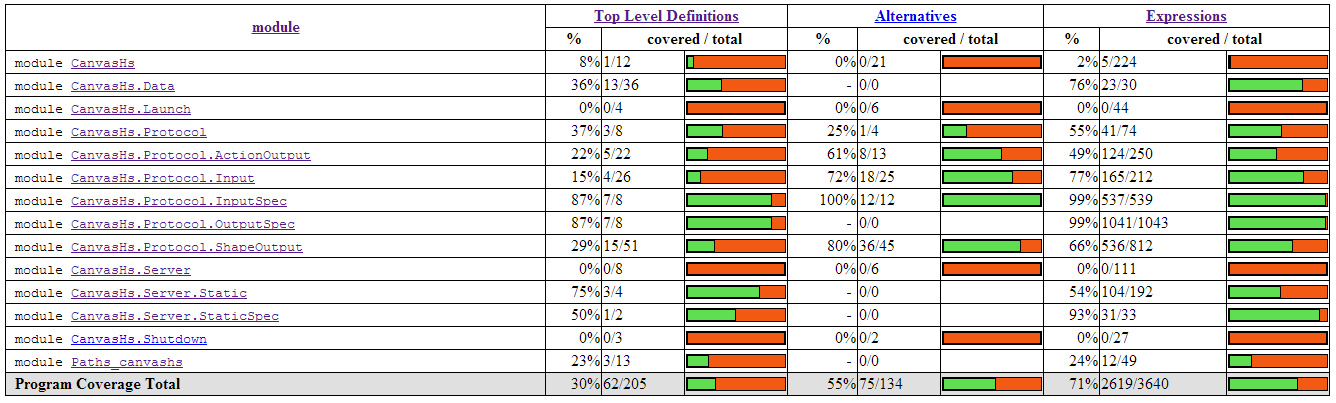
\includegraphics[keepaspectratio,width=\textwidth]{./images/haskellcoverage.png}
\caption{Code coverage resultaten uit HPC}
\label{fig:hpc}
\end{center}
\end{figure}

De code coverage resultaten die uit een analyse van HPC komen zijn niet direct uit te drukken in één compleet getal. Zoals te zien is in \autoref{fig:hpc}, zijn er verschillende onderdelen van de code die gemeten worden, namelijk: de definieties, alternatieven en expressies. Bij het evalueren van de resultaten kijken wij naar de expressies van de modules die relevant zijn voor het gegevensmodel. Zo zijn de test-modules zelf meegenomen in de resultaten, maar deze zijn deze resultaten niet relevant. Daarnaast zijn modules die te maken hebben met I/O en randzaken ook niet meegenomen in onze beoordeling aangezien het lastig is hiervoor betrouwbare tests te schrijven.

We kijken specifiek naar de \inlinecode{CanvasHs.Data}, \inlinecode{CanvasHs.Input}, \inlinecode{CanvasHs.Output}, \inlinecode{CanvasHs.ActionOutput} en \inlinecode{CanvasHs.ShapeOutput}. Hier komt het neer op 848 geteste expressies van de 1304. Dat is een resultaat van 65 \% code coverage voor de geschreven relevante Haskell-code.

\subsection{Gebruiksvriendelijkheid API}
Voor de gebruiksvriendelijkheid van de API hebben we requirements opgesteld. Dit zijn requirements die getoetst worden op het feit of de implementatie hieraan voldoet of niet, er is geen test voor uit te voeren.

\begin{enumerate}[label={T\arabic*}]
	\setcounter{enumi}{\value{startvaluetest}}
	\item \label{test:opzet:monadisch} Alle functionaliteit die aangeboden wordt door Canvas.hs aan de gebruiker maakt geen gebruik van monadische constructies en voldoen daarmee aan \ref{req:monadisch}.
	\item \label{test:opzet:modulair} Canvas.hs is modulair opgebouwd en bezit over voldoende documentatie zodat latere uitbreidingen makkelijk toegevoegd kunnen worden aan de code. Hierdoor voldoet Canvas.hs aan \ref{req:maintenance}.
\end{enumerate}

\subsection{Traceability matrix} \label{sec:traceability}
De traceability matrix laat zien of alle requirements getest zijn. Wanneer een requirement niet getest is betekent dit dat de functie niet geimplementeerd is of dat er geen test voor bestaat. Met de traceability matrix kan bijgehouden worden of alle functionaliteiten geimplementeerd zijn. Om de traceability matrix enigszins overzichtelijk te houden zijn alleen een deel van de testcases opgenomen in de matrix.

\begin{figure}
\begin{center}
\resizebox{\linewidth}{!}{\begin{tabular}{cc|c|c|c|c|c|c|c|c|c|c|c|c|c|c|c|c|c|c|c|c|c|c|c|c|c|c|c|c|c|c|c|c|c|}
\cline{3-29}
& & \multicolumn{27}{ |c| }{Requirements} \\ \cline{3-29}
& & \ref{req:prim}  &
\ref{req:circle} &
\ref{req:rect} &
\ref{req:lines} &
\ref{req:bezier} &
\ref{req:text} &
\ref{req:pictures} &
\ref{req:colors:lines} &
\ref{req:colors:fill} &
\ref{req:colors:fill:gradient} &
\ref{req:event:key} &
\ref{req:event:mouse} &
\ref{req:event:scroll} &
\ref{req:action:animate} &
\ref{req:zoom} &
\ref{req:action:prompt} &
\ref{req:action:fullscreen} &
\ref{req:action:localfiles} &
\ref{req:action:userfiles} &
\ref{req:errors} &
\ref{req:launchbrowser} &
\ref{req:reload} &
\ref{req:debug} &
\ref{req:multiplatform} &
\ref{req:performance} &
\ref{req:maintenance} &
\ref{req:coverage}  \\ \cline{1-29}
\multicolumn{1}{|c|}{\multirow{4}{*}{Tests}} & \ref{test:js:convert:rgbajson:rgba} 		&   &   &   &   &   &   &   &   &   &   &   &   &   &   &   &   &   &   &   &   &   &   &   &   &   &   &		 \\ \cline{2-29}
\multicolumn{1}{|c|}{} & \ref{test:js:execute:actions:displayfixed}						&   &   &   &   &   &   &   &   &   &   &   &   &   &   &   &   & X &   &   &   &   &   &   &   &   &   &		 \\ \cline{2-29}
\multicolumn{1}{|c|}{} & \ref{test:js:execute:actions:displayfluid}						&   &   &   &   &   &   &   &   &   &   &   &   &   &   &   &   & X &   &   &   &   &   &   &   &   &   &		 \\ \cline{2-29}
\multicolumn{1}{|c|}{} & \ref{test:js:execute:actions:opencontrol}						&   &   &   &   &   &   &   &   &   &   &   &   &   &   &   &   &   &   &   & X &   &   &   &   &   &   &		 \\ \cline{2-29}
\multicolumn{1}{|c|}{} & \ref{test:js:execute:actions:closecontrol}						&   &   &   &   &   &   &   &   &   &   &   &   &   &   &   &   &   &   &   & X &   &   &   &   &   &   &		 \\ \cline{2-29}
\multicolumn{1}{|c|}{} & \ref{test:js:parse:actions:fullscreen}							&   &   &   &   &   &   &   &   &   &   &   &   &   &   &   &   & X &   &   &   &   &   &   &   &   &   &		 \\ \cline{2-29}
\multicolumn{1}{|c|}{} & \ref{test:js:convert:rgbajson:rgba}							&   &   &   &   &   &   &   & X & X &   &   &   &   &   &   &   &   &   &   &   &   &   &   &   &   &   &		 \\ \cline{2-29}
\multicolumn{1}{|c|}{} & \ref{test:js:convert:rgbajson:rgba:alphazero}					&   &   &   &   &   &   &   & X & X &   &   &   &   &   &   &   &   &   &   &   &   &   &   &   &   &   &		 \\ \cline{2-29}
\multicolumn{1}{|c|}{} & \ref{test:js:convert:rgbjson:rgba} 							&   &   &   &   &   &   &   & X & X &   &   &   &   &   &   &   &   &   &   &   &   &   &   &   &   &   &		 \\ \cline{2-29}
\multicolumn{1}{|c|}{} & \ref{test:js:draw:line}, \ref{test:haskell:line}				& X &   &   & X &   &   &   &   &   &   &   &   &   &   &   &   &   &   &   &   &   &   &   &   &   &   &		 \\ \cline{2-29}
\multicolumn{1}{|c|}{} & \ref{test:js:draw:rect}, \ref{test:haskell:rect}				& X &   & X &   &   &   &   &   &   &   &   &   &   &   &   &   &   &   &   &   &   &   &   &   &   &   &		 \\ \cline{2-29}
\multicolumn{1}{|c|}{} & \ref{test:js:draw:polygon}, \ref{test:haskell:polygon}			& X &   &   &   &   &   &   &   &   &   &   &   &   &   &   &   &   &   &   &   &   &   &   &   &   &   &		 \\ \cline{2-29}
\multicolumn{1}{|c|}{} & \ref{test:js:draw:arc}, \ref{test:haskell:arc}					& X &   &   &   &   &   &   &   &   &   &   &   &   &   &   &   &   &   &   &   &   &   &   &   &   &   &		 \\ \cline{2-29}
\multicolumn{1}{|c|}{} & \ref{test:js:draw:circle}, \ref{test:haskell:circle}			& X & X &   &   &   &   &   &   &   &   &   &   &   &   &   &   &   &   &   &   &   &   &   &   &   &   &		 \\ \cline{2-29}
\multicolumn{1}{|c|}{} & \ref{test:js:draw:circle:alpha} 								& X & X &   &   &   &   &   &   &   &   &   &   &   &   &   &   &   &   &   &   &   &   &   &   &   &   &		 \\ \cline{2-29}
\multicolumn{1}{|c|}{} & \ref{test:js:draw:text}, \ref{test:haskell:text}				& X &   &   &   &   & X &   &   &   &   &   &   &   &   &   &   &   &   &   &   &   &   &   &   &   &   &		 \\ \cline{2-29}
\multicolumn{1}{|c|}{} & \ref{test:js:draw:container}, \ref{test:haskell:containers}	& X &   &   &   &   &   &   &   &   &   &   &   &   &   &   &   &   &   &   &   &   &   &   &   &   &   &		 \\ \cline{2-29}
\multicolumn{1}{|c|}{} & \ref{test:js:draw:container:clipping} 							& X &   &   &   &   &   &   &   &   &   &   &   &   &   &   &   &   &   &   &   &   &   &   &   &   &   &		 \\ \cline{2-29}
\multicolumn{1}{|c|}{} & \ref{test:js:mouse}, \ref{test:haskell:mouse}					&   &   &   &   &   &   &   &   &   &   &   & X &   &   &   &   &   &   &   &   &   &   &   &   &   &   &		 \\ \cline{2-29}
\multicolumn{1}{|c|}{} & \ref{test:js:mouse:draw} 										&   &   &   &   &   &   &   &   &   &   &   & X &   &   &   &   &   &   &   &   &   &   &   &   &   &   &		 \\ \cline{2-29}
\multicolumn{1}{|c|}{} & \ref{test:haskell:scroll} 										&   &   &   &   &   &   &   &   &   &   &   &   &   &   &   &   &   &   &   &   &   &   &   &   &   &   &		 \\ \cline{2-29}

\multicolumn{1}{|c|}{} & \ref{test:blackbox:keyevents}	 								&   &   &   &   &   &   &   &   &   &   & X &   &   &   &   &   &   &   &   &   &   &   &   &   &   &   &		 \\ \cline{2-29}
\multicolumn{1}{|c|}{} & \ref{test:blackbox:scrollevents}								&   &   &   &   &   &   &   &   &   &   &   &   & X &   &   &   &   &   &   &   &   &   &   &   &   &   &		 \\ \cline{2-29}


\multicolumn{1}{|c|}{} & \ref{test:blackbox:prompt}										&   &   &   &   &   &   &   &   &   &   &   &   &   &   &   & X &   &   &   &   &   &   &   &   &   &   &		 \\ \cline{2-29}
\multicolumn{1}{|c|}{} & \ref{test:blackbox:lokalebestanden}							&   &   &   &   &   &   &   &   &   &   &   &   &   &   &   &   &   & X &   &   &   &   &   &   &   &   &		 \\ \cline{2-29}
\multicolumn{1}{|c|}{} & \ref{test:blackbox:animatie}									&   &   &   &   &   &   &   &   &   &   &   &   &   & X &   &   &   &   &   &   &   &   &   &   &   &   &		 \\ \cline{2-29}
\multicolumn{1}{|c|}{} & \ref{test:blackbox:download}, \ref{test:haskell:download}		&   &   &   &   &   &   &   &   &   &   &   &   &   &   &   &   &   &   & X &   &   &   &   &   &   &   &		 \\ \cline{2-29}
\multicolumn{1}{|c|}{} & \ref{test:blackbox:upload} 									&   &   &   &   &   &   &   &   &   &   &   &   &   &   &   &   &   &   & X &   &   &   &   &   &   &   &		 \\ \cline{2-29}
\multicolumn{1}{|c|}{} & \ref{test:blackbox:error} 										&   &   &   &   &   &   &   &   &   &   &   &   &   &   &   &   &   &   &   & X &   &   &   &   &   &   &		 \\ \cline{2-29}
\multicolumn{1}{|c|}{} & \ref{test:blackbox:debug} 										&   &   &   &   &   &   &   &   &   &   &   &   &   &   &   &   &   &   &   &   &   &   & X &   &   &   &		 \\ \cline{2-29}
\multicolumn{1}{|c|}{} & \ref{test:blackbox:multiplatform} 								&   &   &   &   &   &   &   &   &   &   &   &   &   &   &   &   &   &   &   &   &   &   &   &   & X &   &		 \\ \cline{2-29}
\multicolumn{1}{|c|}{} & \ref{test:blackbox:browser} 									&   &   &   &   &   &   &   &   &   &   &   &   &   &   &   &   &   &   &   &   &   &   &   &   &   & X &		 \\ \cline{2-29}
\multicolumn{1}{|c|}{} & \ref{test:blackbox:coverage} 									&   &   &   &   &   &   &   &   &   &   &   &   &   &   &   &   &   &   &   &   &   &   &   &   &   &   & X	 	 \\ \cline{2-29}
\end{tabular}}
\caption{Traceability matrix, zie \autoref{sec:traceability}}
\label{fig:traceability}
\end{center}
\end{figure}





